\documentclass[submission,copyright]{eptcs}
\providecommand{\event}{WWV 2012}
\usepackage{breakurl}

\usepackage[utf8]{inputenc} % set input encoding (not needed with XeLaTeX)

\usepackage{graphicx} % support the \includegraphics command and options

%%% PACKAGES
\usepackage{booktabs} % for much better looking tables
\usepackage{array}    % for better arrays (e.g. matrices) in maths
\usepackage{paralist} % very flexible & customisable lists (eg. enumerate/itemize, etc.)
\usepackage{verbatim} % adds environment for commenting out blocks of text & for better verbatim
\usepackage{subfig}   % make it possible to include more than one captioned figure/table in a single float
\usepackage{listings}
\usepackage{xspace}

%%% HEADERS & FOOTERS
\usepackage{fancyhdr} % This should be set AFTER setting up the page geometry
\pagestyle{fancy} % options: empty , plain , fancy
\renewcommand{\headrulewidth}{0pt} % customise the layout...
\lhead{}\chead{}\rhead{}
\lfoot{}\cfoot{\thepage}\rfoot{}

\lstset{language=erlang,
        basicstyle=\footnotesize\ttfamily,
        columns=flexible,
        %tabsize=2,
        %numberbychapter=false,
        captionpos=b,
        %commentstyle=,
        %basewidth=0.51em,
        frame=single,
        %framesep=2pt,
        %frameround=tttt,
        breaklines=true,
        breakatwhitespace=true}

\newcommand{\LET}{\texttt{?LET}\xspace}

\title{Automatic WSDL-guided Test Case Generation\\
       for Property-Based Testing of Web Services}
\author{Leonidas Lampropoulos \and Konstantinos Sagonas}
\def\titlerunning{Automatic WSDL-guided Test Case Generation for Property-Based Testing of Web Services}
\def\authorrunning{L. Lampropoulos and K. Sagonas}

\begin{document}
\maketitle

\begin{abstract}
With web services already being key ingredients of modern web systems,
automatic and easy-to-use but at the same time powerful and expressive
testing frameworks for web services are increasingly important. Our
work aims at fully automatic property-based testing of web services:
ideally the user only specifies properties that the web service is
expected to satisfy, in the form of input-output relations, and the
system handles all the rest. In this paper we present in detail the
component which lies at the heart of this system: how the WSDL
specification of a web service is used to automatically create test
case generators that can be fed to PropEr, a QuickCheck-like
property-based testing tool, to create structurally valid random
test cases for its operations. Although the process is fully automatic,
our tool optionally allows the user to easily modify its output to
either add semantic information to the generators or write properties
that test for more involved functionality of the web services.
\end{abstract}


\section{Introduction}

% Web services + their testing

Web Services are an essential part of modern web systems, especially
since the appearance of the Service-Oriented Architecture (SOA).
Testing Web Services, however, is an extremely slow and painful
process, mainly due to the overly verbose nature of XML SOAP messages
which makes writing testcases by hand not a practical option. Many of
the existing tools for testing web services help speed up this
process, up to a point, but when the web service functionality becomes
involved, they fail to assist the tester in testing the Web Services
in an easy and straightforward manner.

% Property based testing + PropEr

One approach that could be used to make the testing of involved web
services easier is property-based testing (PBT). The idea of PBT is to
express the properties that a program must satisfy in the form of
input-output relations, and present the general structure of valid
input messages, while letting the system handle the creation of
progressively more complex testcases to try to find a counter-example
for the property. Property-based testing is gaining popularity,
especially in the community of functional programming where tools such
as QuickCheck (for Haskell and Erlang) or PropEr (for Erlang) exist.
%
Property-based testing applied to web services shares the same problem
as other testing approaches: the generators would be most cumbersome
to write manually. This is where our tool comes in: It automatically
creates test case generators and simple properties to be tested based
on the WSDL specification of the web service and feeds them to PropEr
for execution. Optionally, it allows their easy modification by the
user in order to test more involved properties that the web service
must satisfy.

% What this paper does + generation techniques

In this paper we describe the methods our tool employs to handle this
automatic test case generation. This idea has already appeared in a
number of papers, however the related tools have yet to mature, while
our design can lead to much deeper and more thorough testing
possibilities because of the integration with PropEr. In addition, we
present some example uses of these generators in automatically testing
web services for unexpected behaviors.

% Paper outline

The rest of the paper is organized as follows.
The next section presents the system architecture of our tool and
reviews its key components: PropEr, Yaws, and xmerl.
Section~\ref{sec:automatic} describes the techniques used to handle
automatic creation of test case generators and properties, along with
some examples to show the form of the output code.
In Section~\ref{sec:response_testing}, we show how to use our tool to
test a single operation of a web service, fully automatically.
Section~\ref{sec:related} compares our work with related research and
tools already available, while the last section draws conclusions and
presents ideas for future work.

\section{System Architecture} \label{sec:architecture}

Figure~\ref{fig:architecture} shows the architecture of our testing
framework. Given a URI, the testing starts by obtaining the WSDL
specification of the web service. This specification is then fed into
two different Erlang tools, Yaws and xmerl, which will be briefly
described later on in this section. Using xmerl we extract all the
type information associated with the WSDL specification, while using
Yaws we extract needed information for all supported (SOAP)
operations. These two pieces of information are then used to create a
testing file (Erlang code) that contains PropEr generators and
properties ready for use. Then, the user can (optionally) modify the
testing file to add his own properties or refine the generators. The
testing file is then given as input to PropEr, which generates random
testcases, invokes the Web service (using Yaws as a SOAP wrapper) and
then analyzes the result.

\begin{figure}
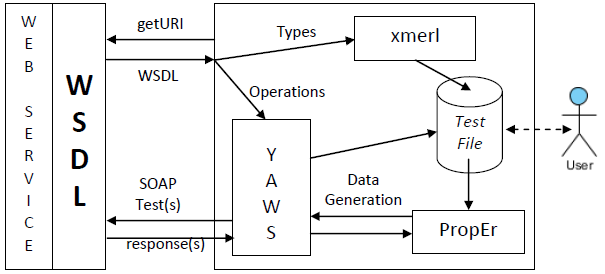
\includegraphics{Framework.png}
\caption{System architecture of our property-based testing framework.}
\label{fig:architecture}
\end{figure}

\subsection{WSDL}

WSDL is the leading specification for web services in XML
format~\cite{wsdl_spec}, describing the web service in full:
operations, input and output message types, locations, bindings, port
types, etc.

Every WSDL specification contains (or references) an XSD schema
inside, describing the types of the messages needed to invoke the web
service~\cite{xsd_structure_spec,xsd_datatypes_spec}. The types of
these messages are divided in two large categories: simple and complex
types. Simple types can be either primitive data types, such as
floats, ints, strings, etc., aggregates of the above, such as lists
and unions, or restricted versions of them, like enumerations or
range-constrained ints. Complex types on the other hand are derived
(extended or restricted) based on other types, which in turn are
either simple or complex. Usually, complex types are created by
forming element aggregates - sequences or choices.

In addition to types, a WSDL specification also describes the operations the 
web service provides, along with information linking the input and output 
messages of an operation with types defined in the XSD Schema. 

\subsection{PropEr}

Property-based testing is a relatively new approach to software
testing. The user specifies the general structure of valid inputs,
together with properties expected to hold about the input-output
relation. PropEr~\cite{proper_tool} is a PBT tool that can receive
this information and create progressively more complex test cases,
execute them and then monitor the response to make sure it conforms
with the specified properties. In addition, should a failing test case
occur, PropEr will try to locate the part of the test case that is
actually responsible for the fault by simplifying (shrinking) the
original test case. Since properties are written in the host language
(Erlang), the user can utilize all of its expressivity to succesfully
describe a vast range of input-output relations.

To use PropEr for web service testing, we first need to specify the structure
of the SOAP messages that will be used to invoke the web service operations. 
Then we need a property that will receive the web service's response and use 
it for validation. Both of these, are handled by our tool. By parsing the 
WSDL specification we create valid PropEr generators, while a sample property
is created, that tests that no exceptions (SOAP Faults) happened and that the 
XML response was well formed.


\subsection{Yaws}

Yaws is the most widely used Erlang HTTP webserver~\cite{yaws}. Yaws
uses an XML parser called Erlsom to handle the encoding and decoding
of SOAP messages, a parser module faster and more user friendly than
the xmerl module of the Erlang distribution, imposing however a few
additional limitations. In our framework, Yaws is used at two
different times: in the beginning, in order to extract all the
supported SOAP operations from the WSDL specification, and during the
actual testing phase, as an intermediary between PropEr and the web
service, wrapping the data generated by PropEr in a valid SOAP
structure, invoking a web service operation with the formed SOAP
message, retrieving the result and returning it in the form of an
Erlang tuple to PropEr for further analysis.

\subsection{xmerl}

Xmerl is an XML parser, included in the Erlang/OTP distribution~\cite{xmerl}.
It transforms any XML to a (rather verbose) Erlang structure containing all the 
information contained in the original XML document. In our framework, xmerl is 
used to parse the XSD Schema of the WSDL specification into an Erlang structure, in 
order to extract afterwards the typing information needed to create PropEr generators.

\section{Automatic Creation of Generators and Properties} \label{sec:automatic}

\subsection{Automatic Creation of Test Case Generators from WSDL Types}

At the heart of our tool lies the automatic creation of PropEr generators from 
the types described in the WSDL specification. To that end, we introduce an 
intermediate Erlang representation of the WSDL types; a representation that can 
be directly mapped to PropEr generators, while at the same time is easier to work 
with and can be used to handle all constraining facets of the XSD Schema. 

Using an XSD schema, one can describe increasingly complex types by combining
smaller, simple datatypes into complex ones. Therefore, the first step towards 
creating the intermediate representation (IR) is mapping the primitive datatypes 
into Erlang tuples. The following table shows this mapping for some of the
most used basic types:

\begin{center}\footnotesize
  \begin{tabular}{cc}
    \toprule
    Simple Type & Erlang IR\\
    \midrule
    boolean & \texttt{$\{$erlsom\_bool, bool, []$\}$}\\
    float & \texttt{$\{$erlsom\_string, float, $\{$inf,inf$\}\}$}\\
    double & \texttt{$\{$erlsom\_string, float, $\{$inf,inf$\}\}$}\\
    integer & \texttt{$\{$erlsom\_string, integer, $\{$inf, inf$\}\}$}\\
    nonPositiveInteger & \texttt{$\{$erlsom\_string, integer, $\{$inf, 0$\}\}$}\\
    negativeInteger & \texttt{$\{$erlsom\_string, integer, $\{$inf, -1$\}\}$}\\
    long & \texttt{$\{$erlsom\_string, integer, $\{$-1 bsl 63, 1 bsl 63 -1$\}\}$}\\
    int & \texttt{$\{$erlsom\_int, integer, $\{$-1 bsl 31, 1 bsl 31 - 1$\}\}$}\\
    short & \texttt{$\{$erlsom\_string, integer, $\{$-1 bsl 15, 1 bsl 15 - 1$\}\}$}\\
    byte & \texttt{$\{$erlsom\_string, integer, $\{$-1 bsl 7, 1 bsl 7 - 1$\}\}$}\\
    nonNegativeInteger & \texttt{$\{$erlsom\_string, integer, $\{$0, inf$\}\}$}\\
    positiveInteger & \texttt{$\{$erlsom\_string, integer, $\{$1, inf$\}\}$}\\
    unsignedLong & \texttt{$\{$erlsom\_string, integer, $\{$0, 1 bsl 64 - 1$\}\}$}\\
    unsignedInt & \texttt{$\{$erlsom\_string, integer, $\{$0, 1 bsl 32 - 1$\}\}$}\\
    unsignedShort & \texttt{$\{$erlsom\_string, integer, $\{$0, 1 bsl 16 - 1$\}\}$}\\
    unsignedByte & \texttt{$\{$erlsom\_string, integer, $\{$0, 1 bsl 8 - 1$\}\}$}\\
    string & \texttt{$\{$list, $\{\{$range, 0, inf$\}$, $\{$erlsom\_int, integer, $\{$32,127$\}\}\}\}$}\\
    \bottomrule
  \end{tabular}
\end{center}

The above format allows us to handle most facets - like the min/max facets - 
simply by altering the related values according to the schema. In addition, the
same list tuple is used to combine elements inside complex structures, when
their \texttt{(minOccurs,maxOccurs)} attributes are different than~\texttt{(1,1)}.

Another important issue that needs addressing is how to combine these simple
datatypes into complex ones. In an XSD schema, there are three main combinators for
this: any, sequence and choice. The following table shows how to create a
complex type. We assume we have the name of the complex type in the 
\texttt{TypeName} variable, and the generators of the ``elements'' of the complex
type in the \texttt{Generators} variable. 

\begin{center}\footnotesize
  \begin{tabular}{cc}
    \toprule
    Indicator & Erlang IR\\
    \midrule
    all & \texttt{$\{$TypeName, $\{$tuple, Generators$\}\}$}\\
    sequence & \texttt{$\{$TypeName, $\{$tuple, Generators$\}\}$}\\
    choice & \texttt{$\{$TypeName, $\{$union, Generators$\}\}$}\\
    \bottomrule
  \end{tabular}
\end{center}

This intermediate representation can be easily mapped to Erlang code. In the 
following table we see how most of the IR tuples representing simple types are
mapped to code:
\begin{center}\footnotesize
  \begin{tabular}{cc}
    \toprule
    Erlang IR & Code\\
    \midrule
    \texttt{$\{$\_, integer, $\{$inf, inf$\}\}$} & \texttt{integer()}\\
    \texttt{$\{$\_, integer, $\{$Min, Max$\}\}$} & \texttt{integer(Min, Max)}\\
    \texttt{$\{$\_, float, $\{$inf, inf$\}\}$} & \texttt{float()}\\
    \texttt{$\{$\_, float, $\{$Min, Max$\}\}$} & \texttt{float(Min, Max)}\\
    \texttt{$\{$\_, bool, \_$\}$} & \texttt{union([true, false])}\\
    \bottomrule
  \end{tabular}
\end{center}

The first argument is one of \texttt{erlsom\_int, erlsom\_string, erlsom\_bool}.
This argument is used afterwards to wrap the resulting code inside a \LET
macro if needed like this:

\begin{center}
  \texttt{?LET(Gen, Code, \%type\%\_to\_list(Gen))}
\end{center}
which converts the generated instance to a string - if Yaws expects it as such.

\subsection{Example}

The following XSD Schema is an example of a type specification of a web service 
which we will use to show how the generators are created.

\begin{lstlisting}
  <complexType name="ProductType">
    <sequence>
      <element maxOccurs="1" minOccurs="1" name="name" type="xsd:string"/>
      <element maxOccurs="1" minOccurs="1" name="price" type="xsd:positiveInteger"/>
      <element maxOccurs="1" minOccurs="1" name="shipInfo" type="impl:ShipInfo"/>
    </sequence>
  </complexType>
  <simpleType name="PaymentType">
    <restriction base="xsd:string">
      <enumeration value="visa"/>
      <enumeration value="paypal"/>
      <enumeration value="deposit"/>
    </restriction>
  </simpleType>
  <complexType name="ShipInfo">
    <sequence>
      <element maxOccurs="1" minOccurs="1" name="paymentInfo" type="impl:PaymentType"/>
      <element maxOccurs="1" minOccurs="1" name="address" type="xsd:string"/>
    </sequence>
  </complexType>
  <element name="Order">
    <complexType>
      <sequence>
        <element maxOccurs="unbounded" minOccurs="1" name="products" type="impl:ProductType"/>
      </sequence>
    </complexType>
  </element>
  <element name="Product" type="impl:ProductType"/>
\end{lstlisting}

% Na mpei edw kapoia perigrafi tou parapanw sximatos i den xreiazetai?

Suppose we want to create a generator for an operation \texttt{"placeOrder"} of a 
web service that takes as an argument a single element \texttt{"Order"}. In the 
front end of the implementation, we use the information provided by the xmerl 
module after parsing the schema to go through all elements and their types recursively, 
passing through all the nodes of the XSD schema in a DFS (depth-first search) style. In every such node, 
we create a tuple that contains both name and type information for the node and 
all its successors. 

Simple types yield tuples that contain only type information, along with an atom 
to facilitate compatibility with Erlsom and Yaws. In our example, we encounter 
three different simple types. Two of them, namely \texttt{xsd:string} and
\texttt{xsd:positiveInteger} represent primitive datatypes of the WSDL specification,
whereas \texttt{tns:PaymentType} is a user defined simple type: a restriction
upon the string type. The tuples associated with these types in our tool are:

\begin{lstlisting}
xsd:positiveInteger : {erlsom_string, integer, {1, inf}}
\end{lstlisting}

The \texttt{positiveInteger} primitive datatype is mapped by default to the
above tuple.  Its first element, the Erlang atom \texttt{erlsom\_string}, states
that for compatibility with Yaws it must be converted to String before wrapped
in a valid SOAP structure, its second element states that the base PropEr
generator is \texttt{integer()}, and the last denotes the range $[1,+\infty)$. 

\begin{lstlisting}
xsd:string : {list, {{range, 0, inf}, {erlsom_int, integer, {32, 127}}}}
\end{lstlisting}

This simple type shows how strings are mapped to intermediate tuples. The first 
element shows that the entire tuple represents a list and the second argument 
specifies the length of the list (in this case it is arbitrary) and the inner type 
(its intermediate representation) of the list (in this case a character - since 
strings in Erlang are lists of numbers, the generator creates such lists with 
integers in the range 32--127, printable characters in the ASCII table).

\begin{lstlisting}
tns:PaymentType: {elements, ["visa", "paypal", "deposit"]}
\end{lstlisting}

The final simple type is a user defined restriction upon the basic
string datatype, defining an enumeration of the acceptable values. As
a result the only acceptable values are \texttt{"visa"},
\texttt{"paypal"} or \texttt{"deposit"} and the intermediate tuple
denotes just that.

Elements yield tuples that contain type and naming information. The
naming information contains the name of the element (if it exists) as
well as namespace information of the XSD Schema. For example the
\texttt{"price"} element:
\begin{lstlisting}
<element maxOccurs="1" minOccurs="1" name="price" type="xsd:positiveInteger"/>
\end{lstlisting}
is represented with the tuple:
\begin{lstlisting}
{{price,['ProductType'],'http://bar'}, {erlsom_string,integer,{1,inf}}}
\end{lstlisting}

Finally complex types usually define aggregates of simple types. In
our example, we encounter three complex types, all of which combine
child elements with a \texttt{sequence} combinator - other options
would include \texttt{all} or \texttt{choice}. For example, the
\texttt{"ShipInfo"} complex type is represented as:

\begin{lstlisting}
{{'ShipInfo',[],'http://bar'},
  {tuple,
    [{{paymentInfo,['ShipInfo'],'http://bar'},
      {{'PaymentType',[],'http://bar'},
       {elements,["visa","paypal","deposit"]}}},
     {{address,['ShipInfo'],'http://bar'},
      {list, {{range,0,inf}, {erlsom_int,integer,{32,127}}}}}]}}
\end{lstlisting}

This shows that besides the name information, the intermediate representation consists of a 
\texttt{tuple} atom - indicative of the \texttt{sequence} combinator - and a list of the 
child intermediate tuples. In this case, since the minOccurs and maxOccurs attributes for 
the child elements are both equal to 1, we include the child generator as is. In case these
attributes implied a collection (e.g., unbounded), we would need to wrap the inner generators 
inside another list generator.

% Back end now

The mapping of the intermediate tuples to PropEr generators is pretty straightforward by design. 
Special care is only needed to ensure names for all generators are unique. To that end we use 
the full path up to the current node as prefix, leading to rather long but descriptive and unique 
names. The generators produced for the previous example by our tool are:

\begin{lstlisting}
generate_Order_1_products_ProductType_name() -> 
  list(integer(32, 127)).

generate_Order_1_products_ProductType_price() ->  
  ?LET(Gen, integer(1,inf), integer_to_list(Gen)).

generate_Order_1_products_ProductType_shipInfo_ShipInfo_paymentInfo_PaymentType() -> 
  elements(["visa", "paypal", "deposit"]).

generate_Order_1_products_ProductType_shipInfo_ShipInfo_address() -> 
  list(integer(32, 127)).

generate_Order_1_products_ProductType_shipInfo_ShipInfo() -> 
  ?LET(
    {Pr_Order_1_products_ProductType_shipInfo_ShipInfo_paymentInfo_PaymentType,
     Pr_Order_1_products_ProductType_shipInfo_ShipInfo_address},
    {generate_Order_1_products_ProductType_shipInfo_ShipInfo_paymentInfo_PaymentType(),
     generate_Order_1_products_ProductType_shipInfo_ShipInfo_address()},
    [Pr_Order_1_products_ProductType_shipInfo_ShipInfo_paymentInfo_PaymentType,
     Pr_Order_1_products_ProductType_shipInfo_ShipInfo_address]
  ).

generate_Order_1_products_ProductType() -> 
  ?LET(
    {Pr_Order_1_products_ProductType_name, 
     Pr_Order_1_products_ProductType_price, 
     Pr_Order_1_products_ProductType_shipInfo_ShipInfo},
    {generate_Order_1_products_ProductType_name(), 
     generate_Order_1_products_ProductType_price(), 
     generate_Order_1_products_ProductType_shipInfo_ShipInfo()},
    [Pr_Order_1_products_ProductType_name, 
     Pr_Order_1_products_ProductType_price, 
     Pr_Order_1_products_ProductType_shipInfo_ShipInfo] 
  ).

generate_Order_1_products() -> 
  ?LET(Len, range(1, inf), vector(Len, generate_Order_1_products_ProductType())).

generate_Order_1() -> 
  ?LET(Pr_Order_1_products, generate_Order_1_products(), [Pr_Order_1_products]).
\end{lstlisting}

The above code reveals the generation method. Simple types are mapped almost directly 
like the \texttt{"PaymentType"}, with special care taken if needed to add a wrapper that converts 
the generated data to string if that is required by Yaws. Complex types on the other hand, 
need to be represented as lists for Yaws to accept them, and we use \LET macros to that end. 

% Include the following or not?
PropEr would allow for simplicity to create less verbose versions of these generators 
with a little extra care for unique naming. For example the last generator could have 
been written as:

\begin{lstlisting}
generate_Order_1() ->
  [generate_Order_1_products()].
\end{lstlisting}

While in a small example - like the above - this would appear preferable, it actually makes things more 
difficult for the user, should he want to modify the generated test data or the generators. 
The importance of the \LET macro can be seen in the following example: Suppose a web service 
has an operation that takes as input an element with an ISBN field amongst others (a 
semantically valid ISBN is a unique identifier for a book and consists of 10 single digits, 
the last of which is determined by the previous nine via a congruence). For such a web service, 
our tool would generate code of the following form:
\begin{lstlisting}
generate_opName() ->
  ?LET(
    {Pr_opName_ISBN,
     ...},
    {generate_opName_ISBN(),
     ...},
    [Pr_opName_ISBN,
     ...]
  ).
\end{lstlisting}
where the \texttt{generate\_opName\_ISBN()} generator would create a
10-member list of single digit integers. With a small function that
changes the first digit so that the ISBN congruence is satisfied (e.g.,
ISBNize()), one could rewrite the generator as:
\begin{lstlisting}
generate_opName() ->
  ?LET(
    {Pr_opName_ISBN,
     ...},
    {generate_opName_ISBN(),
     ...},
    [ISBNize(Pr_opName_ISBN),
     ...]
  ).
\end{lstlisting}

This is only possible with the use of the \LET macro that allows a user to
modify and combine the generated data. 

\subsection{Automatic Creation of Properties from WSDL Operations}

In addition to automatically creating generators, our tool also
creates a couple of functions for each web service operation, that
invokes this operation using Yaws. Also, it creates a small property
to test that the web service always responds for random testcases, with a
well formed SOAP message. This approach allows us to find most basic
errors in a web service implementation identifying SOAP:Fault
structures, since SOAP Faults are analogous to Java exceptions.

For the XSD Schema of the previous section, our tool creates the following code:
\begin{lstlisting}
call_placeOrder(Arguments) ->
  inets:start(),
  WSDL = yaws_soap_lib:initModel(?WSDL_URL),
  yaws_soap_lib:call(WSDL, "placeOrder", Arguments).
    
call_placeOrder(WSDL, Arguments) ->
  yaws_soap_lib:call(WSDL, "placeOrder", Arguments).
\end{lstlisting}
Both functions invoke the \texttt{placeOrder} operation of the
web service feeding \texttt{Arguments} to Yaws to wrap in a SOAP
message. The difference between the two, is that the first function
attempts to start the inets module (an Erlang module that includes an
HTTP client) and also parses the WSDL specification of the web service
in order to create the model Yaws needs in order to make the actual
call. The second function takes the WSDL model of the Web Service as
an argument and invokes the operation directly, thus being more
efficient than the first.

Finally, the property that is automatically created is the following:

\begin{lstlisting}
prop_placeOrder_responds() ->
  ?FORALL(Args, generate_Order_1(),
    begin
      Result = call_placeOrder(Args),
      case Result of 
        {ok, _Attribs, [#'soap:Fault'{}]} -> false;
        {ok, _Attribs, _Result_record} -> true;
        _ -> false
      end
    end).
\end{lstlisting}

The responds property is a \texttt{FORALL} macro, creating random data for the Web Service using 
the PropEr generators previously created, uses the aforementioned calling functions to 
invoke the operation and finally does a pattern matching on the resulting tuple. If Yaws 
encountered some problem in parsing the SOAP messages an \{error, Reason\} tuple is returned
and the property is not satisfied. Also, if a \texttt{soap:Fault} struct is encountered as the 
body of the web service SOAP response, the web service failed to respond correctly and the 
property is also not satisfied. In any other case, Yaws was able to parse a valid SOAP answer, 
so we assume the web service responded correctly and move on to the next testcase. For deeper
result validation the user needs to modify this property (or write another of his own) utilizing
the full power of a host language like Erlang.

For the resulting file to be directly compilable, we include all headers, defines and imports 
needed by Erlang. In addition a function called \texttt{answer\_placeOrder} is created which 
shows how to extract the answer (record) that is returned by Yaws. Finally, the extension also 
uses erlsom to output a small .hrl (Erlang library) file that describes the records used for the 
responses of the Service. This last library file helps the user in decoding the SOAP message 
responses without having to deal with XML parsing.

\section{Response Testing of Web Services} \label{sec:response_testing}

One kind of testing our tool can handle, that works without any user additions is response testing. Basically, 
the output file created by the extension contains a property that invokes an operation of the 
web service with random inputs and expects an answer for each different input. This can basically 
check if a web service crashes for a specific input or similar unwanted behaviors. 

Let us see how to use the tool to test an existing Web Service that
converts between cooking units. This free Web Service is hosted at
\url{http://www.webservicex.net/ConvertCooking.asmx} and its WSDL
specification lies at
\url{http://www.webservicex.net/ConvertCooking.asmx?WSDL"}.

The XSD Schema of the Web Service is the following:
\begin{lstlisting}
  <s:element name="ChangeCookingUnit">
    <s:complexType>
      <s:sequence>
        <s:element minOccurs="1" maxOccurs="1" name="CookingValue" type="s:double" />
        <s:element minOccurs="1" maxOccurs="1" name="fromCookingUnit" type="tns:Cookings" />
        <s:element minOccurs="1" maxOccurs="1" name="toCookingUnit" type="tns:Cookings" />
      </s:sequence>
    </s:complexType>
  </s:element>
  <s:simpleType name="Cookings">
    <s:restriction base="s:string">
      <s:enumeration value="drop" />
      <s:enumeration value="dash" />
      ...
      <s:enumeration value="TenCan" />
    </s:restriction>
  </s:simpleType>
  <s:element name="ChangeCookingUnitResponse">
    <s:complexType>
      <s:sequence>
        <s:element minOccurs="1" maxOccurs="1" name="ChangeCookingUnitResult" type="s:double" />
      </s:sequence>
    </s:complexType>
  </s:element>
  <s:element name="double" type="s:double" />
\end{lstlisting}
where the \texttt{Cookings} simple type is a large enumeration with
most of the values omitted in the Schema above. Our tool creates the
output file (by default this file is named
\texttt{proper\_output.erl}) which can be used directly to check the
Web Service:

% Change names of functions (wsdl_handler:generate for instance)?
\begin{lstlisting}
Erlang R15B (erts-5.9) [source] [64-bit] [smp:4:4] [async-threads:0] [hipe] [kernel-poll:false]

Eshell V5.9  (abort with ^G)
1> wsdl_handler:generate("http://www.webservicex.net/ConvertCooking.asmx?WSDL").
ok
2> c(proper_output).
{ok,proper_output}
3> proper:quickcheck(proper_output:prop_ChangeCookingUnit_responds()).
....(100 dots) .....
OK: Passed 100 test(s).
true
\end{lstlisting}

As we can see, the Cooking web service was invoked 100 times with random 
arguments and returned a correctly formed result each time.

Now for an example of a service that crashes, we created our own web
service using eclipse and tomcat. This example is a variation of an
example about a faulty \texttt{lists:delete} function given
in the first PropEr publication ~\cite{PropErTypes@Erlang-11}, which we
also used to ensure similar behaviour when testing traditional programs
and web services using PropEr.

We have a simple Java implementation of the web service logic, to make it
directly comparable with the original Erlang implementation:

\begin{lstlisting}
public Class Delete {
    private String delete(String in, char c, StringBuffer acc){
        if (in.equals("")) {
            return acc.toString();
        }
        else if (in.charAt(0) == c) {
            return acc.toString().concat(in.substring(1));
        }
        else {
            return delete(in.substring(1), c, acc.append(in.charAt(0)));
        }
    }
    
    public String delete(String in, String c){
        return delete(in, c.charAt(0), new StringBuffer(""));
    } 
}
\end{lstlisting}

We used this code to implement and publish a simple web service in tomcat. 
After using the PropEr extension to handle the WSDL specification of this 
web service, the output file was the following:

\begin{lstlisting}
-module(proper_output).

-include_lib("proper/include/proper.hrl").
-include("proper_output.hrl").

-define(PREFIX, "properns").
-define(WSDL_URL, "http://localhost:8080/DeleteProject/services/Delete?WSDL").

-export([call_delete/1, call_delete/2]).
-export([answer_delete/1]).

generate_delete_1_in() -> 
  list(integer(32, 127)).

generate_delete_1_c() -> 
  list(integer(32, 127)).

generate_delete_1() -> 
  ?LET({Pr_delete_1_in, Pr_delete_1_c},
       {generate_delete_1_in(), generate_delete_1_c()},
       [Pr_delete_1_in, Pr_delete_1_c]).

call_delete(Arguments) ->
  inets:start(),
  Wsdl = yaws_soap_lib:initModel(?WSDL_URL),
  yaws_soap_lib:call(Wsdl, "delete", Arguments).
    
call_delete(WSDL, Arguments) ->
  yaws_soap_lib:call(WSDL, "delete", Arguments).

prop_delete_responds() ->
  ?FORALL(Args, generate_delete_1(),
    begin
      Result = call_delete(Args),
      case Result of 
        {ok, _Attribs, [#soap:Fault()]} -> false; 
        {ok, _Attribs, _Result_record} -> true;
        _ -> false
      end
    end).

answer_delete({ok, _, [Answer_record]}) -> Answer_record.
\end{lstlisting}

Calling PropEr to quickcheck this property reveals a flaw in our implementation.
\begin{lstlisting}
> proper:quickcheck(proper_output:prop_delete_responds()). 
.!
Failed: After 2 test(s).
[[46],[]]

Shrinking .(1 time(s))
[[],[]]
false
\end{lstlisting}

In our implementation we assume that the string $c$ which is supposed
to contain at its first character the character that should be removed
from the string, is not empty. We have two options of fixing it, either
fix our implementation, or remove this testcase from the generator. To
demonstrate how easy it is to change the generators created by the extension
we choose the latter: we change the generator of $c$ to:
\begin{lstlisting}
generate_delete_1_c() ->
  ?LET(Len, range(1,1), vector(Len, integer(32,127))).
\end{lstlisting}

We could change it to \texttt{range(1,inf)} or actually remove the
\LET macro, but we would need to be careful not to actually change the
output of the generator to a char instead of a non-empty char list.

Now only valid testcases are created. Testing the response property again we 
get:
\begin{lstlisting}
> proper:quickcheck(proper_output:prop_delete_responds()).
....(100 dots) .....
OK: Passed 100 test(s).
true
\end{lstlisting}

\section{Related Work} \label{sec:related}

Research in testing Web Services has seen a lot of growth in the past
few years. A variety of tools has emerged handling disparate aspects
of testing, from functional to integration and regression testing; cf.
a survey on the subject~\cite{SOATesting@springerlink-09}. Our tool
can handle automatic functional testing with structurally valid
testcases created based on the WSDL specification of a web service.
Prior research work using a similar idea includes the work of
Bartolini~\textit{et al.}~\cite{bartolini@ICSOC-08} and of
Zhang~\textit{et al.}~\cite{zhang@IC-08}. Most existing tools have
expanded on the idea of generating XML messages based on a static
analysis of the WSDL specification. Most of them, however, lack in the
aspect of validating the results of the web service and just present
them to the user for inspection.

% Currently similar, goal best? (vevaia to goal psiloiparxei idi sto diko mas)
Amongst the existing frameworks and tools in the area, there are a few that 
stand out. 
Most notably, SoapUI~\cite{soapUI}, one of the most complete testing frameworks
that can handle semi-automated functional testing, amongst other things. This 
tool however does not automatically generate sample test cases, just aids the
user in doing so.
Other tools, such as WSDLTest~\cite{wsdltest@IEEE06} are similar to ours in 
generation strategy, yet user input happens for every script if modifications 
and assertions (for output validation) are needed. Our tool, creates generators 
that allow random test case creation, while any modification by the user to
refine the generators needs to take place only once and will be valid for all
the SOAP messages generated.
Another category of tools is the one that contains WS-Taxi~\cite{taxi@IC-08}. 
This is one of the first tools to have been created based on the idea
of WSDL-based testing. WS-Taxi was first outlined in
2007~\cite{partition@AST-07}, but as stated in the related papers,
while it provides automatic data generation, the tool lacks a test oracle.
%
Finally, there is a couple of papers and a tool that use Haskell's
QuickCheck to do automatic test case generation. The idea
in~\cite{ws_quickcheck} is largely similar to our own: to create
generators for a PBT tool to allow for automatic testing. The tool
that spawned from this effort, monadWS~\cite{monadWS@AST-11}, contains
a promising comparison with SoapUI and SoapTest, yet also does not
utilize the power of QuickCheck for deeper validation of the results
returned by the web service.

All in all, what makes our tool stand out from the rest is that it 
was designed for use with a property based testing tools with the 
power of PropEr. Our tool handles automatic test data generation as
efficiently and automatically as many other available tools, yet its
design will allow for faster and powerful testing, using properties 
to automatically validate an arbitrary number of progressively more 
complex testcases.

\section{Concluding Remarks and Future Work}

We demonstrated how our tool can be used to automatically test web services, 
with a different approach than the existing tools on the market. 
% Using our tool, we were able to succesfully test a large number of web services 
% available for free, mostly in webservicex.net. From the 30+ web services we 
% attempted to test, all proved to respond with valid XML for all random inputs 
% provided by PropEr.
One course for future work is to perfect test case generation. Our tool, 
while still under development, can successfully test all free web
services it was tried against, handling most types and constraining
facets appearing in XSD schemas. However, some types that are not
frequently encountered - like some date formats or the pattern
constraining facet - are yet to be handled by our tool and need to be addressed.
Our main goal now, however, is to handle property-based testing of web services 
using our tool and figure out in which areas our tool could aid the user even 
further. Successful PBT would be a huge asset for web service testers, speeding 
up the time needed to create test cases and doing the actual testing 
significantly.

\bibliographystyle{eptcs}
\bibliography{ws}

\end{document}
